\documentclass[12pt]{article}
\usepackage[spanish]{babel}
\usepackage{geometry}
\geometry{a4paper, margin=1in}
\usepackage{graphicx}
\usepackage{xcolor}
\usepackage{titlesec}
\usepackage{parskip}
\usepackage{multicol}
\usepackage{cite}
\usepackage{float}

\definecolor{highlight}{RGB}{255, 255, 0}

\titleformat{\section}{\normalfont\Large\bfseries}{\thesection}{1em}{}
\titleformat{\subsection}{\normalfont\large\bfseries}{\thesubsection}{1em}{}

\begin{document}

% Logos
\begin{minipage}{0.45\textwidth}
    
\includegraphics[width=0.4\textwidth]{inFiles/Figures/epnLogo.jpg}
\end{minipage}
\hfill
\begin{minipage}{0.45\textwidth}
    \raggedleft
    
\includegraphics[width=0.4\textwidth]{inFiles/Figures/FIS_logo.jpg}
\end{minipage}

\vspace{0.5cm}

% Títulos principales
\begin{center}
    \textbf{ESCUELA POLITÉCNICA NACIONAL}\\[0.2cm]
    \textbf{FACULTAD DE INGENIERÍA DE SISTEMAS}\\[0.2cm]
    \textbf{INGENIERÍA {\textbf{EN COMPUTACIÓN}}}
\end{center}

\vspace{0.5cm}
\hrule
\vspace{0.5cm}

% Datos principales
\noindent\textbf{PERÍODO ACADÉMICO:} 2025-A\\[0.2cm]
\noindent\textbf{ASIGNATURA:} ICCD412 Métodos Numéricos \hfill \textbf{GRUPO:} GR2\\[0.2cm]
\noindent\textbf{TIPO DE INSTRUMENTO:} Tarea 5\\[0.2cm]
\noindent\textbf{FECHA DE ENTREGA LÍMITE:} 04/05/2025\\[0.2cm]
\noindent\textbf{ALUMNO:} Murillo Tobar Juan

\vspace{0.5cm}
\hrule
\vspace{1cm}


% Secciones
\section*{TEMA}
Método de la bisección

\vspace{0.5cm}

\section*{OBJETIVOS}
\begin{itemize}
    \item Comprender la utilidad del método de bisección para la búsqueda de ceros(soluciones) dentro de un intervalo en donde la función es continua.
    \item Determinar el error producido al momento de utilizar el método de bisección y relacionarlo con el objetivo de los métodos numéricos.
\end{itemize}

\vspace{0.5cm}

\section*{MARCO TEÓRICO}

\large\textbf{Método de la bisección}
\normalsize\newline\newline
Es un método numérico, es decir, encuentra una solución al problema de forma aproximada. El problema a resolver utilizando este método es encontrar las raíces o soluciones para una ecuación de la forma $f(x) = 0$.
Como se menciona en \cite{book:2608618}, es una técnica también conocida como método de búsqueda binaria y se basa en teorema del valor intermedio. Este método consiste a la reducción sucesiva a la mitad de los subintervalos hasta aproximarnos a la raíz dentro de ese intervalo, ya que como se enuncia en el teorema del valor intermedio, dentro de un intervalo [a, b] con f(a) y f(b) con signo opuesto, dadas estas condiciones existirá un p dentro de [a,b] tal que f(p) = 0. Ademas, debemos recordar que la función en dicho intervalo debe ser continua para considerar dicho teorema. 
\vspace{0.5cm}

\section*{DESARROLLO}
\large\textbf{CONJUNTO DE EJERCICIOS 2.1}
\normalsize\newline
\textbf{1}.Use el método de bisección para encontrar soluciones precisas dentro de $10^{-2}$ para la función $x^3 -7x^2 +14x-6$, en cada intervalo.
\newline\textbf{a) $[0, 1]$}
\begin{center}
    \begin{tabular}{|c|c|c|c|c|c|c|}
        \hline
        a & b&p&$f(a)$&$f(b)$&$f(p)$&$E_{est}$\\
        \hline
        0 & 1&  0.5& -6& 2& -0.625& 0.5\\
        0.5 & 1&  0.75& -0.625& 2& 0.984375& 0.25\\
        0.5 & 0.75&  0.625& -0.625& 0.984375& 0.259765& 0.125\\
        0.5 & 0.625&  0.5625& -0.625& 0.259765& -0.161865& 0.0625\\
        0.5625 & 0.625&  0.59375& -0.161865& 0.259765& 0.0540466& 0.03125\\
        0.5625 & 0.59375&  0.578125& -0.161865& 0.054046& -0.0526237& 0.015625\\
        \hline
      \end{tabular} 
\end{center}


\textbf{b) $[1, 3.2]$}
\begin{center}
    \begin{tabular}{|c|c|c|c|c|c|c|}
        \hline
        a & b&p&$f(a)$&$f(b)$&$f(p)$&$E_{est}$\\
        \hline
        1       & 3.2      &  2.1    &  2       & -0.112  & 1.791    & 1.1\\
        2.1     & 3.2     &  2.65    & 1.791    & -0.112  & 0.552125  & 0.55\\
        2.65    & 3.2   &  2.925     & 0.552125   & -0.112  & 0.0858281  & 0.275\\
        2.925   & 3.2  &  3.0625     & 0.0858281   & -0.112& -0.0544434 & 0.1375\\
        2.925   & 3.0625  &  2.99375 & 0.0858281& -0.0544434& 0.00632788 & 0.06875\\
        2.99375 & 3.0625&  3.02813   & 0.00632788& -0.0544434& -0.0265251& 0.034375\\
        2.99375 & 3.02813&  3.01094  & 0.00632788& -0.0265251& -0.0106993& 0.01719\\
        \hline
      \end{tabular} 
\end{center}

\textbf{c) $[3.2, 4]$}
\begin{center}
    \begin{tabular}{|c|c|c|c|c|c|c|}
        \hline
        a & b&p&$f(a)$&$f(b)$&$f(p)$&$E_{est}$\\
        \hline
        3.2      & 4      &  3.6     & -0.112       & 2       & 0.336    & 0.4\\
        3.2    & 3.6      &  3.4    & -0.112   & 0.336       & -0.016  & 0.2\\
        3.4    & 3.6   &  3.5   & -0.016   & 0.125& 0.125  & 0.1\\
        3.4    & 3.5  &  3.45  & -0.016   & 0.259765& 0.046125 & 0.05\\
        3.4 & 3.45  &  3.425 & -0.016& 0.046125& 0.0130156 & 0.025\\
        3.4 & 3.425&  3.4125& -0.016& 0.0130156& -0.00199805& 0.0125\\
        \hline
      \end{tabular} 
\end{center}


\textbf{2.a}.Dibuje las gráficas mencionadas 

\begin{figure}[H]
    \centering
    \begin{minipage}{0.5\textwidth}
        \centering
        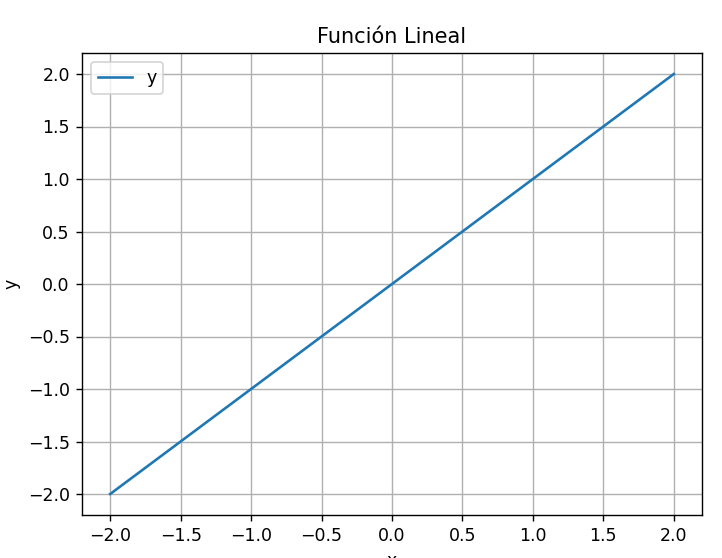
\includegraphics[width=0.9\textwidth]{./inFiles/Figures/Cap1.png}
        \caption{Gráfica \( y = x \)}
    \end{minipage}%
    \begin{minipage}{0.5\textwidth}
        \centering
        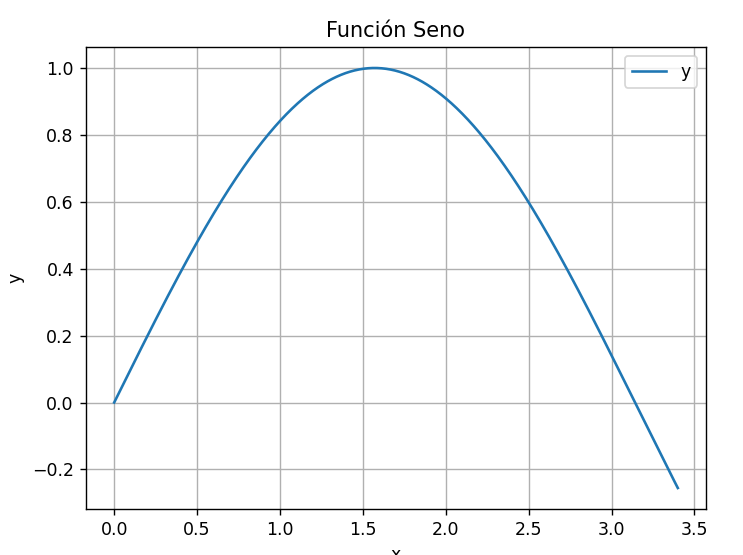
\includegraphics[width=0.9\textwidth]{./inFiles/Figures/Cap2.png}
        \caption{Gráfica \( y = \sin(x) \)}
    \end{minipage}
\end{figure}

\textbf{2.b}.Use el método de bisección para encontrar soluciones precisas dentro de $10^{-5}$ para el primer x positivo de la función $2\sin(x) - x$, en cada intervalo.

En este caso sabemos que para dicha función el primer corte positivo sera en $x \approx 1.89549$ por lo que definimos un intervalo cercano que contenga dicho valor como [1.89541, 1.89550]
y comenzamos a realizar el método de bisección. Aclarar que el cálculo debe ser en radianes.
\begin{center}
    \begin{tabular}{|c|c|c|c|c|c|c|}
        \hline
        a & b&p&$f(a)$&$f(b)$&$f(p)$&$E_{est}$\\
        \hline
        1.89541    & 1.89550 &  1.89546     & $1.38026*10^{-4}$& $-9.39089*10^{-6}$& $5.61298*10^{-5}$  & $4.5*10^{-5}$\\
        1.89546    & 1.89550 &  1.89548     & $5.61298*10^{-5}$& $-9.39089*10^{-6}$& $2.33699*10^{-5}$  & $2*10^{-5}$\\
        \hline
      \end{tabular} 
\end{center}

\textbf{3.a}.Dibuje las gráficas mencionadas 

\begin{figure}[H]
    \centering
    \begin{minipage}{0.5\textwidth}
        \centering
        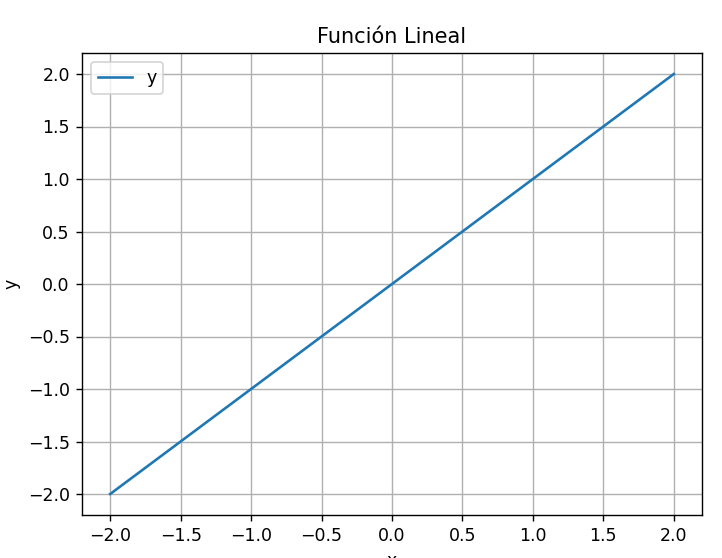
\includegraphics[width=0.9\textwidth]{./inFiles/Figures/Cap1.png}
        \caption{Gráfica \( y = x \)}
    \end{minipage}%
    \begin{minipage}{0.5\textwidth}
        \centering
        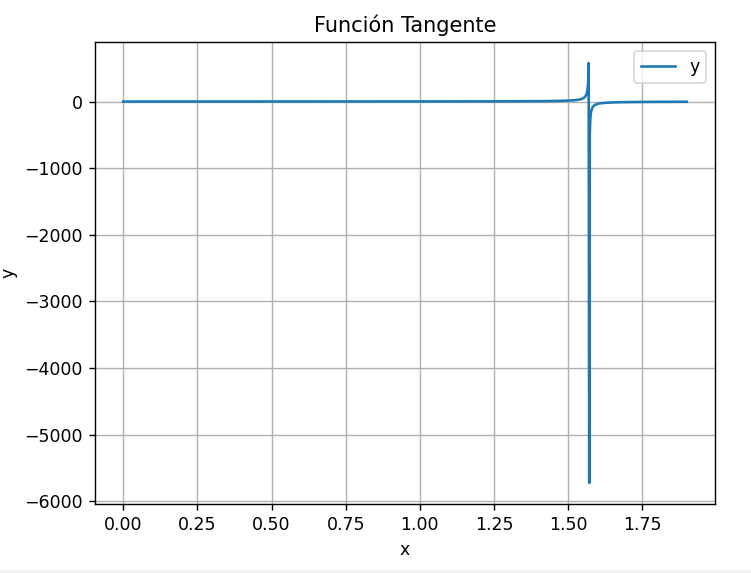
\includegraphics[width=0.9\textwidth]{./inFiles/Figures/Cap4.png}
        \caption{Gráfica \( y = \tan(x) \)}
    \end{minipage}
\end{figure}

\textbf{3.b}.Use el método de bisección para encontrar soluciones precisas dentro de $10^{-5}$ para el primer x positivo de la función $\tan x - x$, en cada intervalo.

En este caso sabemos que para dicha función el primer corte positivo sera en $x \approx 4.493409$ por lo que definimos un intervalo cercano que contenga dicho valor como [4.49330, 4.49342]
y comenzamos a realizar el método de bisección. 


\begin{center}
    \begin{tabular}{|c|c|c|c|c|c|c|}
        \hline
        a & b&p&$f(a)$&$f(b)$&$f(p)$&$E_{est}$\\
        \hline
        4.49330    & 4.49342  &  4.49336        & $-2.20889*10^{-3}$& $2.12863*10^{-4}$ & $-9.98358*10^{-4}$ & $6*10^{-5}$\\
        4.49336    & 4.49342  &  4.49339        & $-9.98358*10^{-4}$& $2.12863*10^{-4}$ & $-3.92833*10^{-4}$ & $3*10^{-5}$\\
        4.49339    & 4.49342  &  4.49341        & $-3.92833*10^{-4}$& $2.12863*10^{-4}$ & $1.09452*10^{-5}$  & $1.5*10^{-5}$\\
        \hline
      \end{tabular} 
\end{center}
\textbf{4.a}.Dibuje las gráficas mencionadas 

\begin{figure}[H]
    \centering
    \begin{minipage}{0.5\textwidth}
        \centering
        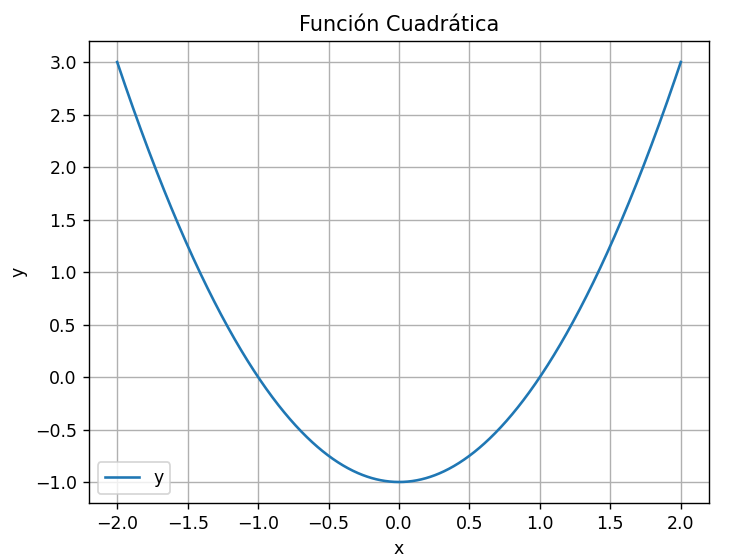
\includegraphics[width=0.9\textwidth]{./inFiles/Figures/Cap5.png}
        \caption{Gráfica \( y = x^2-1 \)}
    \end{minipage}%
    \begin{minipage}{0.5\textwidth}
        \centering
        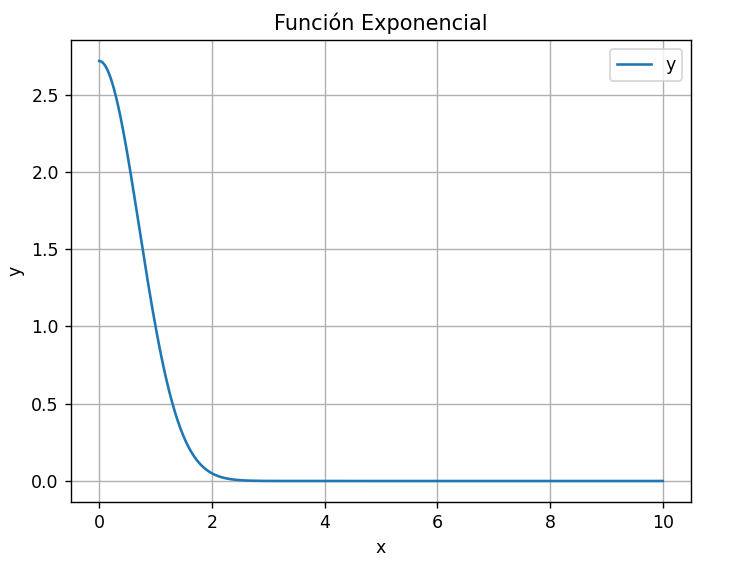
\includegraphics[width=0.9\textwidth]{./inFiles/Figures/Cap6.png}
        \caption{Gráfica \( y = \exp(1-x^2) \)}
    \end{minipage}
\end{figure}

\textbf{4.b}.Use el método de bisección para encontrar soluciones precisas dentro de $10^{-5}$ para el primer x positivo de la función $e^{1-x^2}-x^2+1$, en cada intervalo.

En este caso sabemos que para dicha función el primer corte positivo sera en $x \approx 1.251856$ por lo que definimos un intervalo cercano que contenga dicho valor como [1.25184, 1.25187]
y comenzamos a realizar el método de bisección. 

\begin{center}
    \begin{tabular}{|c|c|c|c|c|c|c|}
        \hline
        a & b&p&$f(a)$&$f(b)$&$f(p)$&$E_{est}$\\
        \hline
        1.25184    & 1.25187  &  1.25186        & $6.25370^{-5}$& $-5.51733*10^{-5}$ & $-1.59365*10^{-5}$     & $1.5*10^{-5}$\\
        \hline
      \end{tabular} 
\end{center}

\textbf{5}. ¿En qué cero de f converge el método de bisección cuando se aplica en los siguientes intervalos?. Siendo $f = (x+2)(x+1)^2x(x-1)^3(x-2)$

Para dar respuesta a cada literal nos fijaremos en cada factor de la función para obtener todas sus raíces, obteniendo que:
$x_1 = -2, x_2 = -1,  x_3 = 0, x_4 = 1, x_5 = 2$

\textbf{a [-1.5, 2.5]}.
\normalsize\newline
Convergiría en $x_2 = -1,  x_3 = 0, x_4 = 1, x_5 = 2$

\textbf{b [-0.5, 2.4]}.
\normalsize\newline
Convergiría en $x_3 = 0, x_4 = 1, x_5 = 2$

\textbf{c [-0.5, 3]}.
\normalsize\newline
Convergiría en $x_3 = 0, x_4 = 1, x_5 = 2$

\textbf{d [-3, -0.5]}.
\normalsize\newline
Convergiría en $x_2 = -1,  x_3 = 0, x_4 = 1, x_5 = 2$, es decir en todas las raíces de la función. 

\vspace{0.5cm}


\renewcommand{\refname}{\MakeUppercase{REFERENCIAS}}
\bibliographystyle{IEEEtran}
\bibliography{inFiles/References/references.bib}

\end{document}
